\chapter{Příprava} \label{swordfightingIntroChapter}
V této kapitole uvedeme čtenáře do problematiky boje s chladnou zbraní - velmi stručně nastíníme jeho vývoj a metodiku v reálném světě a následně do hloubky rozebereme mechaniky, skrze které ho adaptuje svět akčních videoher, a problémy, které při tom musí řešit.


\section{Chladná zbraň v reálném světě}
V této sekci čtenáře velmi stručně seznámíme s historickým pozadím a základními charakteristikami, které provázejí boj s chladnou zbraní v reálném světě.

\subsection{Průlet historií}

Není nadsázkou když prohlásíme, že chladná zbraň je koncept starý jako lidstvo samo. Archelogické nálezy nasvědčují, že již vzdálený předek moderního člověka Australopithecus používal úderný předmět (pravděpodobně kus dřeva či kost ulovené antilopy) jako \textbf{nástroj k lovu} paviánů \cite{AustralopithecusWeapon}. \textbf{Výhody}, které mu to mohlo přinést, jsou zjevné: zatímco kořist měla možnosti obrany omezené tím, kam dosáhly její vlastní zuby a drápy, lovec si ji mohl držet v bezpečné vzdálenosti a vystavovat vlastní tělo o poznání menšímu nebezpečí odvety.

V průběhu svého vývoje lidský rod zdokonaloval i své zbraně, což přineslo mnoho dalších implikací - ostrý kamenný hrot člověku umožnil zasazovat ránu spolehlivě, a hlubší, než by kdy umožnilo pouhé jeho tělo. Spolehlivost zbraně umožnila lepší \textbf{koordinaci mezi lovci}. Sofistikovaná koordinace člověku otevřela cestu k lovu větších a silnějších druhů zvěře. Nakonec se člověk propracoval na samý vrchol potravního řetězce a zbraň, nástroj lovu, sloužila stále více pro vzájemný \textbf{boj mezi lidmi}. 

Zrod civilizací vznesl na zbraň nové požadavky. Vysoká koncentrace lidí na jednom místě vedla přirozeně ke specializaci profesí, mezi jinými i vojenské. \textbf{Profesionální armáda} čítající tisíce lidí umožňovala (a vyžadovala) do té doby nevídanou míru koordinace - ideálem v takové situaci se ukázalo disponovat širokou škálou zbraní vysoce specializovaných, chladných i střelných, jež mohly být použity ve vzájemné synergii, doplněné válečnými stroji a vhodně vycvičenými zvířaty\footnote{kůň jak známo hrál přední roli}. Profesionální voják měl čas a motivaci svůj typ zbraně pochopit do hloubky, stejně tak vysoce náročná si mohla dovolit být i její výroba a údržba, za níž nesli zodpovědnost rovněž profesionálové ve svém oboru. 
Na druhé straně tu však byl \textbf{běžný obyvatel}, který nepatřil k pravidelnému vojenskému jádru, ale byla-li říše pod útokem, považovalo se za samozřejmost, že pozvedne zbraň na její obranu. Zbraň pro takového člověka vyžadovala především jednoduchost - jak na výrobu, tak na údržbu a použití, zkrátka aby bylo možné v časové tísni krizové situace dostat co nejrychleji co nejvíce odvedenců do bojeschopného stavu a udržet je v něm.

Mocenské soupeření států ústí ve zběsilý a nikdy nekončící \textbf{závod ve vývoji účinnějších zbraní a metod jejich použití}. V jednom okamžiku dominuje Blízkému východu vozataj, v následujícím jej poráží Makedonská falanga, nad ní předvede svou superioritu Římský systém manipulů, ten vzápětí Římané sami prohlašují za zastaralý, avšak o půl tisíciletí později stejně jejich říši rozvrací hordy Hunských jezdců... chladná zbraň, ať už v rukou jezdce či pěšího vojáka, zůstává po většinu dějin dominantním prvkem na bojišti, se střelnými zbraněmi hrajícími významnou podpůrnou roli. Až s rozmachem zbraní palných se tato dynamika obrací a velmi pozvolně se dobíráme k modernímu vojenství. V současné době se chladná zbraň považuje převážně za překonanou - uplatnění pro ní stále existuje např. v kontextu pořádkových složek, avšak i pro ty plní úlohu spíše doplňkovou. Mimo oficiální kruhy pořád hraje nezanedbatelnou roli, avšak to je především pro její \textbf{triviální dostupnost} v porovnání s palnou zbraní.

Tradice chladné zbraně však stále žije v civilních komunitách dedikovaných zachování historie a kulturního odkazu. Mezi významné patří japonské umění \textbf{Kendó} (''cesta meče'') vycházející ze samurajské tradice, či evropská komunita \textbf{historického šermu}, jež vychází z dochovaného učení středověkých mistrů. Rovněž je zde moderní \textbf{sportovní šerm}, jež přímo navazuje na šermířskou tradici ranného novověku. V posledních letech tyto vlivy více pronikají i do běžných volnočasových aktivit - ve Střední Evropě například je stále oblíbenější fenomén \textbf{LARP}\footnote{\ac{LARP}}, jehož jedna z podob - tzv. ''dřevárna'' - znamená hromadnou akci, na které se desítky až stovky lidí v tématických kostýmech a vyzbrojení zpravidla dřevěnými, molitanem měkčenými replikami zbraní, střetnou v bitvě. Pravidla přirozeně musí zaručit bezpečí účastníků, avšak stále při zachování autentického zážitku z boje.  

Vzhledem k charakteru a rozšířenosti výše zmíněných fenoménů lze očekávat, že jejich zastánci mají v nemalé míře zastoupení i ve videoherní komunitě. Přirozeně takoví lidé mohou mít zájem o hru, jež jim umožní jejich oblíbenou činnost napodobit, ale bez mnohých nepohodlí, jež ji provázejí v reálném světě. Pro hráče, který s bojem v reálném světě žádnou zkušenost nemá, může zase videohra být cestou, jak tuto mezeru ve svých zkušenostech částečně zaplnit a získat například hlubší porozumění k historii.

\subsection{Průběh boje}
Nyní si představíme typický průběh boje vedeného s chladnými zbraněmi, a vypíchneme na něm znaky, které by videohra měla dokázat vystihnout, pokud se pokouší o realistický bojový systém.
\bigbreak

Cílem souboje je v nejjednodušším případě protivníka \textbf{zabít, vážně zranit či ho jinak vyřadit z bojeschopného stavu}, čehož může být dosaženo libovolnými prostředky, a ideálně zabránit, aby při tom stejný úděl potkal i vás. Není vyloučeno vítězství vyčerpáním protivníka či využití okolních předmětů a znalosti prostředí (např. lstivým vlákáním protivníka do bažiny).

Tato absolutní svoboda však může být omezena morálními zásadami účastníků\cite{HistoryOfSurrender} či předem dohodnutými pravidly souboje. Velmi zde záleží na \textbf{okolnostech}, při kterých k boji dochází:
\begin{itemize}
    \item Např. při \textbf{obraně domácnosti} před vetřelcem platí popis výše
    \item \textbf{Voják v bitvě} koná v mezích, jež mu stanovuje vojenská disciplína a rozkazy velitele
    \item \textbf{Účastník turnaje} přirozeně nesmí opustit vyhrazené bojiště či využívat pomoci z publika
    \item Ve \textbf{cvičném souboji} si účastníci logicky dávají pozor, aby jeden druhého zbytečně nezabil či nezmrzačil
    \item V duelu na obranu cti se účastníci mohli \textbf{předem dohodnout}, že nechtějí jeden druhého zabít, a např. bojovat ''na první krev''
\end{itemize}
Mezi znaky zkušeného šermíře patří schopnost být si vědom těchto mantinelů a v jejich rámci jednat kreativním a účinným způsobem.

Extrémní případ těchto omezení vidíme v moderních šermířských komunitách. U těch najdeme velmi \textbf{striktní pravidla} a vysoké nároky na bojovou výstroj s cílem zamezit jakýmkoliv vážným zraněním a ztrátám na životech, jelikož ty přirozeně nejsou cílem jejich snažení. 

Avšak pokud nedochází k žádným reálným zraněním, \textbf{jak lze rozhodnout, kdo vyhrál?} Zjevnou cestou je například systém zásahových zón a počítání životů, které se bojovníkovi v závislosti na zasažené zóně odečítají. Takový systém však nezaručuje realistický dojem z boje. Mezi plody snah o realističtější zážitek patří např. v české LARPové scéně oblíbený šatrh\cite{Satrh}, založený na důvěře v účastníky, že podle způsobu, jakým byli zasaženi, odhadnou a zahrají realistickou reakci, či buhurt, kde zkrátka vítězí ten, kdo nepadne vyčerpáním. Je tedy vidět, že i komunity, jejichž nejvyšší prioritou při boji je záruka bezpečí, jsou ochotné vyvinout značnou snahu, aby byl zážitek z boje realistický.

\subsection{Boj jeden na jednoho}
Jak tedy probíhá duel mezi dvěma šermíři? Hloubkový rozbor zohledňující historické i moderní techniky, rozdílné úrovně zkušenosti, zdatnosti a motivace obou zápasníků, veškeré obvyklé zbraně, kterými by mohli být vybaveni, prostředí a vnější okolnosti, které v souboji mohou hrát podstatnou roli, není možné provést v rozsahu bakalářské práce, natož jedné její kapitoly. Pro ten tedy čtenáře odkáži na specializovanou literaturu \cite{KunstDesFechtens} \cite{FightingWithTheGermanLongsword} \cite{ModernHEMA}.  

Zde si pouze nastíníme pár základních faktorů, které při souboji hrají důležitou roli.

\textbf{Obratnost zbraně} - schopnost rychle měnit její trajektorii, reagovat na změny situace (např. vyblokovat nečekaný úder) či změny situace sám vyvolat (např. na poslední chvíli zastavit fingovaný úder a stočit čepel na jiné místo, které protivník nechal nechráněné). Mezi faktory, kterými je determinována, patří velikost a hmotnost zbraně, její tvar, těžiště a způsob úchopu\footnote{Čím jsou ruce dál od sebe, tím silnější je princip páky.}; v neposlední řadě také síla a tělesné rozpoložení šermíře.

\textbf{Dosah, pohyb, terén} - V okamžiku, kdy vám protivník není schopen ublížit a vy jemu ano, můžete si dovolit být libovolně agresivní\footnote{Díky tomu dlouhé zbraně jako kopí mohou být velmi účinné i v rukou nezkušeného odvedence.}. Je-li váš protivník v takovéto výhodě, jedinou možností je se k němu přiblížit - pak se dostanete do výhody vy, jelikož zbraně s dlouhým dosahem zpravidla trpí na nízkou obratnost při boji zblízka\footnote{Nedejte protivníkovi čas tasit poboční zbraň.}. Vaše možnosti, jak se k němu přiblížit, přirozeně velmi závisí na terénu\footnote{Když stojíte pod hradbami a protivník bodá kopím z ochozu nad vámi, jste v pěkné kaši.}. 

Máte-li jeden druhého v dosahu, pohyb se však nestává o nic méně důležitým. Správná technika pohybu pomáhá šermíři držet pod kontrolou jeho těžiště a nenechat se rozhodit, když klopýtne, či na něj protivník agresivně naběhne; případně mu umožní bleskově se přiblížit a využít nechráněnou oblast, kterou mu protivník nabídl svým nemotorným pohybem. 

\textbf{Zbroj}, kterou má protivník na sobě, může citelně omezit vaše možnosti co do způsobů, jak mu uštědřit zranění. Je-li například v plné plátové zbroji pozdního středověku, pokoušet se do ní sekat mečem je prakticky zbytečné. Vaše možnosti se citelně zúží - buď se můžete pokusit bodnout do některé ze skulin ve zbroji, nebo meč vyměnit za palcát či válečné kladivo\footnote{Případně lze meč chytit za čepel a záštitou zasuplovat hlavici kladiva - viz \cite{FightingWithTheGermanLongsword}} a protivníkovi tupými údery pochroumat vnitřnosti a zlámat kosti. Protivník si vaší situace bude vědom, a o to jednodušší pro něj bude předvídat vaše akce.

Znakem každého dobrého šermíře je schopnost vcítit se do pozice svého protivníka a \textbf{odhadovat jeho budoucí akce} dříve, než se stanou. Nezkušený šermíř bude každý svůj úder provázet výrazným nápřahem, pro jeho protivníka pak není obtížné úder vyblokovat a přitom se rovnou k protivníkovi přiblížit a seknout po místě, které ví, že při úderu protivník nechal nechráněné. Zkušený šermíř pak ani nepotřebuje vidět výrazný nápřah, naučí se protivníkovu akci podvědomě vycítit z drobných náznaků (pohybů svalů, očí,...). Samozřejmě je možné předvádět údery fingovaně a čekat, že se při protiútoku otevře protivník vám. Pak záleží na jeho úsudku, zda úmysl prokoukne a provede fingovaný protiútok - stupňům falše se meze nekladou. 


\begin{figure}[ht]\centering
    \center
    \includegraphics[width=140mm]{../img/Meyer_1570_Sword_B.png}
    \includegraphics[width=140mm]{../img/Meyer_1570_Sword_C.png}
    \caption{Průběh souboje: techniky pro jedenapůlruční meč - Joachim Meyer (1570) \cite{KunstDesFechtens}}
    \label{obr01:KunstDesFechtens}
    
\end{figure}

\subsection{Hromadný boj a boj proti přesile} \label{organizedFightingIrlSubsection}
Souboj jeden na jednoho však může vypadat jako téměř laboratorní podmínky vedle chaotických situací, v rámci kterých v historii běžně k boji docházelo.   

Často se střetávaly větší, více či méně \textbf{organizované skupiny}, případně celé armády čítající mnoho takových pevně ustanovených jednotek. V takové situaci je na místě, aby bojovníkova individualita ustoupila do pozadí - rozhodujícím faktorem je až na výjimky taktické jednání a sladěnost celku. 

Jedním ze základních požadavků, které jsou na vojáka kladeny, je schopnost \textbf{držení formace}. Stojíte-li jako semknutá řada, štít na štít, meče připravené opětovat jakýkoliv úder, který by protivník zkusil na kamaráda vedle, je mnohem těžší prorazit vašimi řadami a dostat se k lučištníkům, kteří nepříteli způsobují těžké ztráty. 

Při skupinové šarvátce hraje zpravidla rozhodující roli taktická \textbf{koordinace} spolubojovníků. Nepřítel, který vám překvapivě vpadl do zad, je mnohem nepříjemnější záležitost, než nepřítel, který postává opodál a čeká, až na něj přijde řada.  

Pro dosažení koordinace je však nutná \textbf{komunikace}. Dohodnout se při šarvátce na postupu, v omezeném čase a aniž by plán byl zachycen protivníkem, vskutku není triviální problém. V kontextu větší bitvy pak důležitost i obtížnost komunikace nabývá zcela nového rozměru a jde o těžký problém, který až do vynálezu moderní vysílačky nebyl uspokojivě vyřešen. Vojenská taktika si vyžaduje flexibilní reakce na změny situace na bojišti, informace musí proudit mezi vojenskými jednotkami a velitelstvím, které jsou často netriviálně fyzicky vzdálené. Jednou možností, jak informaci předat, je vyslání posla - ten je schopen nést detailní informaci, je však zranitelný a pomalý - než dorazí, může již jeho informace být neaktuální. Protipólem pak je broadcast předem dohodnutých signálů, napříkald prostřednictvím trubače - tato cesta je rychlá a v určitém doslechovém okruhu vcelku spolehlivá, avšak signály musí být předem dohodnuté a variant nemůže být mnoho, metoda tedy postrádá flexibilitu a detailnost informace. Jak vidno, jde o zásadní součást vedení bitvy, přesto však vidíme mnoho videoher (např. \cite{Medieval2TotalWar} \cite{Warcraft3}), které ji zcela zanedbávají.
\bigbreak
Dojde-li k boji \textbf{jediného bojovníka proti přesile}, vše výše uvedené stále platí, akorát očividně kolosální výhody plynoucí z koordinovaného postupu jsou dopřány pouze jedné ze stran. I pro velmi zkušeného šermíře bojujícího proti několika nezkušeným, často jediná šance, jak z takové situace vyváznout, je protivníky rozdělit (kreativním použitím pohybu a znalosti terénu) a zdolat jednoho po druhém rychle, než mu ostatní přijdou na pomoc.

\subsection{Shrnutí}
Chladná zbraň provází lidstvo od samých jeho počátků. V průběhu dějin si metody její výroby a použití prošly bouřlivým vývojem, vzniklo mnoho metodik, mezi nejlépe dochované patří japonské tradiční umění Kendó a učení středověkých evropských mistrů - kolem obou z nich je v dnešní době soustředěna mohutná komunita civilních nadšenců.

Cílem boje je v typickém případě jakýmikoliv prostředky protivníka vyřadit z bojeschopného stavu. Mezi hlavní devizy zkušeného šermíře patří orientace na bojišti, schopnost pohybu, obratné zacházení se zbraní a schopnost předvídání protivníka. V hromadném boji toto stále platí, přednostní význam však přebírá taktické jednání, koordinace a disciplína vojenského celku.

\clearpage
%------------------------------------------------------------------------------------------------------------------------------------------------------------------------------------------------------------------------------------------------------------%
 % xxxxxxxxxxxxxxxxxxxxxxxxxxxxxxxxxxxxxxxxxxxxxxxxxxxxxxxxxxxxxxxxxxxxxxxxxxxxxxxxxxxxxxxxxxxxxxxxxxxxxxxxxxxxxxxxxxxxxxxxxxxxxxxxxxxxxxxxxxxxxxxxxxxxxxxxxxxxxxxxxxxxxxxxxxxxxxxxxxxxxxxxxxxxxxxxxxxxxxxxxxxxxxxxxxxxxxxxxxxxxxxxxxxxxxxxxxxxxxxxxxxxxxxx %
%------------------------------------------------------------------------------------------------------------------------------------------------------------------------------------------------------------------------------------------------------------%


\section{Chladná zbraň v akčních videohrách}

Nyní, když máme rámcovou představu, jak boj s chladnou zbraní vypadá v reálném světě, nastíníme si, jakým způsobem bývá typicky adaptován v akčních videohrách - jaké jeho aspekty se podařilo v tomto universu věrně zpodobnit, jaké byly ignorovány, a jaké interpretovány s řádnou dávkou umělecké kreativity?

\subsection{Obecný přehled} \label{weaponInVideogamesBasics}

Účinkujícími ve hře jsou \textbf{herní postavy}. Ty mohou být ovládané buď hráčem (takovou postavu nazveme \textbf{\acs{PC}}\footnote{\Acl{PC}}), nebo počítačovým algoritmem (tu označíme jako \textbf{\acs{NPC}}\footnote{\Acl{NPC}}), a lze je popsat nějakým jejich \textbf{vnitřním stavem}. Nyní si představíme základní veličiny, které jsou typickou součástí vnitřního stavu postavy ve všech akčních hrách bez ohledu na to, zda jde o hru zaměřenou na boj se střelnou zbraní, chladnou zbraní, či boj jakýkoliv jiný:

\begin{itemize}
    \item \textbf{\ac{HP}}... \linebreak Číslo udávající zdravotní stav a životaschopnost postavy. \textbf{Pokud klesne na nulu, postava umírá.} K jeho snížení může dojít například úderem protivníkovy zbraně či pádem z výšky a takto odebraným bodům HP říkáme \textbf{\acs{dmg}}\footnote{\Acl{dmg}}. Hráči je stav jeho HP obvykle v reálném čase explicitně komunikován skrze ukazatel na obrazovce. V průběhu boje typicky nejsou doplňovány\footnote{Popřípadě prostředky, skrze které je lze doplnit, jsou vzácné.} a postava musí vystačit s tím, co má - jde tedy o zdroj vybízející k dlouhodobějšímu hospodaření.
    \item \textbf{Výdrž}... Volitelný avšak častý prvek, číslo reprezentující akutní schopnost postavy vynakládat fyzické úsilí. Spotřebováváno chvatným pohybem a prováděním akcí, v průběhu boje zpravidla dochází k jeho rychlému opakovanému spotřebování a regeneraci.
    \item \textbf{Inventář}... List dalších předmětů, které postava nese s sebou. Může jít o peníze, léčivé lektvary, munici, náhradní zbraně, magické svitky, mapy a cokoliv dalšího v závislosti na hře. 
\end{itemize}

V závislosti na vstupu, který získává od hráče či od řidícího algoritmu, se postava pohybuje po herním světě, interaguje s objekty herního světa a s obsahem svého inventáře a používá svou zbraň. Na použití zbraně se nyní zaměříme.

\textbf{Ovládání zbraně} bývá typicky omezené na stisknutí tlačítka - \textbf{Zaútoč!} - načež postava sama provede útok tak, jak uzná za vhodné - obvykle přehráním jedné ze seznamu animací, které pro danou kombinaci postavy a zbraně předem připravil autor hry.

Implikace, které takto jednoduché rozhraní přináší \textbf{pro hráče}, jsou následující:
\begin{itemize}
    \item \textbf{Intuitivnost} - Hráč, který poprvé spustí hru a zkusí náhodně mačkat tlačítka, rychle ovládání pochopí a začne být ve hře použitelný - žádná nutnost procházet úmorným tutoriálem.
    \item \textbf{Uniformní rozhraní pro všechny zbraně} - Tímto způsobem lze ovládat libovolnou zbraň, ať už jde o dvoumetrovou halapartnu či pěsti hráčovy postavy. Hráč tedy není přehlcen množstvím jednoúčelových herních systémů a z výhod, které získá svým zdokonalováním v použití bojového systému, může těžit po celou hru.
    \item \textbf{Nízká specifičnost} - Rozhraní hráči neumožňuje těžit ze silných stránek žádné konkrétní zbraně. Hra mu skrze bojový systém není schopna poskytnout vzdělávací lekci ohledně vlastností zbraně v reálném světě. Pokud hráči tyto vlastnosti již jsou známé, může trpět jeho imerze.
    \item \textbf{Limitovaná předvídatelnost} - Vzhledem k tomu, že akci, která bude vykonána, nevybírá hráč, ale jeho herní postava, vnáší se tím do hry prvek náhody, který má potenciál hru emocionálně okořenit.\footnote{Pokud však výběr akce probíhá nějakým deterministickým způsobem, hráč v něm brzy intuitivně vypozoruje určité vzory a naučí se akce své postavy do jisté míry předvídat a kalkulovat s nimi při plánování svého postupu - tím může bojový systém získat na hloubce.}
\end{itemize}

A co důsledky, které tento přístup přináší z pohledu \textbf{tvůrce hry}?:
\begin{itemize}
    \item \textbf{Předvídatelnost} - Tvůrce hry má přesnou kontrolu nad tím, jaké akce může jakákoliv postava potenciálně vykonat. Tím se zmenšuje prostor pro výskyt neošetřených okrajových případů.
    \item \textbf{Uniformní rozhraní pro všechny zbraně} - Herní logika, která umí pracovat s jednou zbraní, umí pracovat s každou zbraní. To může dopomoci k celkově čistému a kvalitnímu kódu a značně se tím snižuje námaha s přidáváním dalších zbraní (či jejich procedurální generací za běhu).
    \item \textbf{Nízká specifičnost} - Není možné uspokojivě ztvárnit veškerá zajímavá specifika konkrétní zbraně. Všechny zbraně se musejí chovat do jisté míry podobně. Často je tak zbraň smrštěna do pouhé tabulky statů\footnote{Povrchní veličiny typu dosah, rychlost úderu, míra způsobeného zranění}.
\end{itemize}

Vidíme, že takovéto pojetí boje se zbraní má mnohá pozitiva, stále je však zřejmé, že \textbf{jde o systém jednoduchý, který sám o sobě nemůže sloužit jako nosná herní mechanika v akční videohře} - žánru, kde cílová hráčská skupina očekává určitou míru komplexity a hloubky.

Hloubka bývá tomuto systému zpravidla dodávána výběrem mezi několika různými typy útoku (každý efektivní v jiné situaci), akcí pro blokování nepřátelských útoků, důrazem na časování (krátkodobé omráčení nepřítele, navazování úderů, odměna za vyblokování nepřítele v přesně správném okamžiku,...) a \textbf{silným propojením s dalšími mechanikami}, jakými je v první řadě pohyb, dále různé lektvary, magie apod. v závislosti na hře.

Toto si nyní názorně předvedeme na příkladě komerčně úspěšné hry z nedávných let.

\subsection{Zaklínač 3 - vzorový příklad}
Zaklínač 3: Divoký Hon \cite{Wiedzmin3} je akční \acs{RPG} hra, která byla vydána r. 2015 polským studiem CD Projekt. Mezi její hlavní důrazy patří \textbf{otevřený fantasy svět}, propracovaný \textbf{nelineární příběh}\footnote{Hra vychází z knižní série Zaklínač Andrzeje Sapkowského \cite{SapkowskiZaklinac}} a v neposlední řadě také dynamický \textbf{bojový systém}.

Hráč se zde ujímá role Geralta z Rivie - zaklínače, \textbf{profesionálního lovce monster}. Ten je kromě svých dvou mečů\footnote{stříbrného pro boj s nestvůrami a železného proti lidem} vybaven flexibilními možnostmi pohybu, jednoduchými kouzly (tzv. Zaklínačská Znamení) a škálou ručně vařených lektvarů. Na své cestě bojuje s lidmi, duchy, upíry, bazilišky i nepopsatelnými obludami z nočních můr.
Jak tedy vypadají mechaniky, skrze které bylo toto vše umožněno?

\begin{figure}[ht]\centering
    \center
    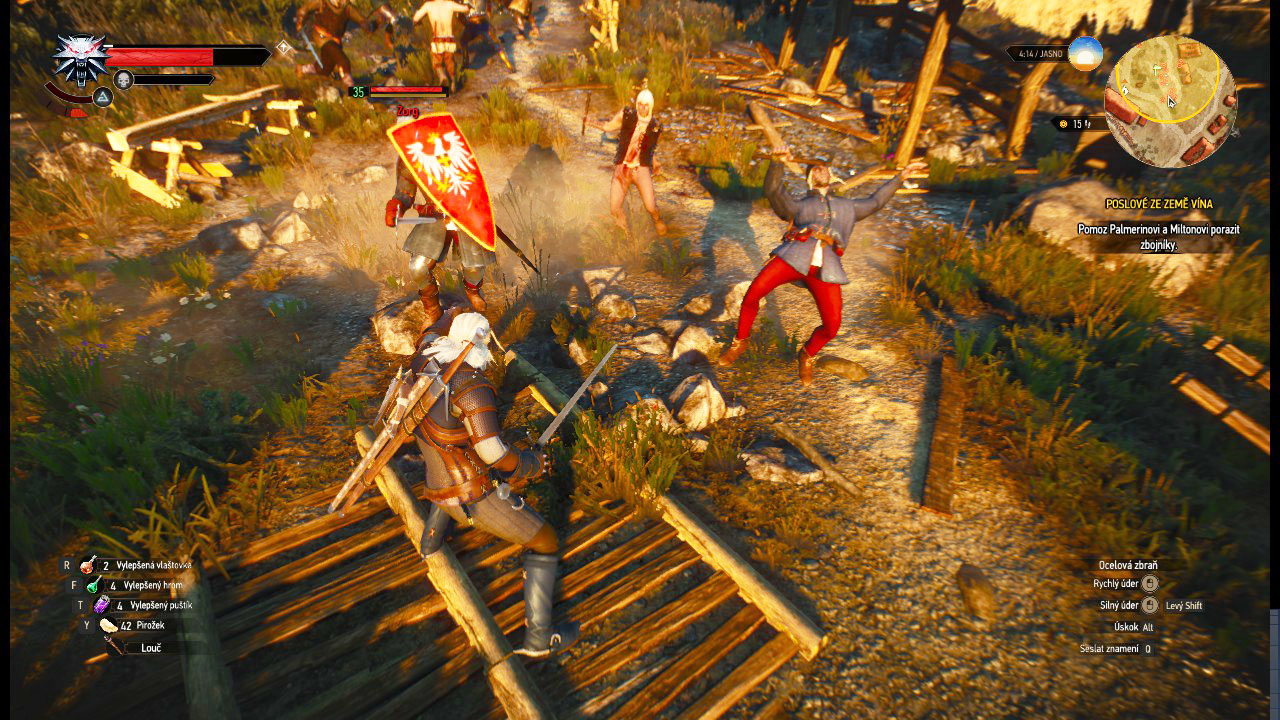
\includegraphics[width=140mm]{../img/Wiedzmin-combat.jpg}
    \caption{Zaklínač 3 - ukázka boje}
    \label{obr01:wiedzmin}
\end{figure} 


Základem jsou \textbf{dva typy úderů - rychlý a silný}. Jak vyplývá z názvu, rychlý úder je rychlejší, oproti tomu animace silného úderu trvá mírně delší čas, avšak zranění způsobené protivníkovi je také adekvátně zvýšené. Jaký z tohoto rozlišení plyne prospěch? Pro mnoho protivníků platí, že v okamžiku, kdy jim je učiněno nezanedbatelné zranění, přeruší akci, kterou se chystali provádět, a na zlomek času zakolísají. S rychlým úderem je hráč schopen toto zakolísání vyvolat častěji - s dobrým časováním se lze například dostat do cyklu, kdy lehkooděného protivníka hráč udolá jedním úderem za druhým aniž ten se zmohl udělat cokoliv proti vám. Toto stejné zakolísání však může potkat i hráče. Hráč se tedy neustále nachází v časovém tlaku, který ho vybízí kalkulovat - např. zda stihne dva rychlé údery, či raději jen jeden silný, než ho nějaký nepřítel přeruší. Dalším důvodem proč používat silný útok jsou těžkoodění nepřátelé, kterým rychlý útok udílí zranění velmi redukované. 

Drobným doplňkem je akce \textbf{blokování}. Bojujete-li proti lidem, držení tlačítka blokování vás činí prakticky imunním proti běžným útokům mířícím na vás zepředu, za tu velmi drobnou cenu, že sám nemůžete útočit a pohybovat se po bojišti lze jen velmi pomalu. Zajímavější je \textbf{perfektní blokování} - pokud zahájíte blokování přesně v okamžiku, kdy na vás protivník vede úder, provedete odvetný protiúder, který protivníka na pár sekund omráčí. Tím je do boje vnesen další prvek časování. Rovněž je třeba dávat pozor na nepřátele, kteří blokují proti vám.
\bigbreak

Proti chaotickým útokům vedeným změtí zubů a drápů nestvůry však blokování mečem ztrácí smysl. Tehdy přicházejí na řadu možnosti úskoků a kotoulů, které nabízí \textbf{systém pohybu}. Kromě nich samozřejmě hra nabízí i klasickou chůzi a sprint. Úskok je velmi drobný posun do strany, který nespotřebovává výdrž, pouze má interní cooldown (několik desetin sekundy) zabraňující spamování. Cílem je umožnit hráči tak akorát uskočit z oblasti dopadu nepřítelovy zbraně. Pro zajištění, že tento záměr bude vždy naplněn, je postavě na malý zlomek sekundy poskytnuta celková nezranitelnost. Kotoul je pak rámcově obdobný s tím rozdílem, že spotřebovává výdrž a na oplátku ho lze použít k rychlému překonání velké vzdálenosti. Hra klade velký důraz na hromadné boje, kde hráč musí být schopen prioritizovat cíle a rychle využívat objevivších se zranitelností jednotlivých nepřátel. Vysoká mobilita, kterou kotoul poskytuje, je tedy více než nápomocná.  

Zaklínačská Znamení do boje přinášejí další vrstvu komplexity. Jde o \textbf{5 kouzel}, která spotřebovávají velkou porci výdrže a na oplátku zaklínači mocně pomohou - např. může jít o ochranné silové pole, poryv větru, který má šanci omráčit zasažené protivníky, či zmatení, které přiměje nepřítele bojovat na vaší straně.

Výčet Znamení je pevně stanoven, avšak klasicky pro žánr \acs{RPG}, hra zahrnuje \textbf{prvky progrese}, pomocí kterých lze Znamení v průběhu hry vylepšovat a modifikovat. Stejné platí i pro boj s mečem - rychlý i silný úder mají každý své vlastní stromy dovedností, které jsou schopny zajímavými způsoby ovlivnit gameplay. 

Poslední částí zaklínačova repertoáru, kterou zmíníme, jsou lektvary a oleje. Jde o \textbf{konzumovatelné předměty}, které hráč v průběhu hry sám vyrábí, a po jejich konzumaci (požití lektvaru postavou / namazání oleje na meč) mu je na určitý časový limit poskytnut nějaký bonus (př. regenerace zdraví, bonusové zranění proti upírům apod.). Jde tedy o zdroje, se kterými hráč hospodaří v dlouhodobějším horizontu, ale použity v kritickém okamžiku mohou zvrátit výsledek boje. 

Esenciální součástí každé hry s bojovými prvky jsou také \textbf{nepřátelé}. V této oblasti byl Zaklínač 3 k hráči velmi štědrý. Najdeme zde obyčejné lidské nepřátele (bandity, nepřátelské vojáky apod.), jejichž způsob boje sdílí mnoho prvků se zaklínačovým - např. jsou schopni blokovat jeho údery. Dále pak širokou paletu monster všech velikostí a tvarů: pozemní i schopné létat vzduchem, vybuchující, duchy zranitelné pouze specifickými cestami, tvory vládnoucí magií - každý nepřítel má své osobité silné a slabé stránky a vybízí hráče k jinému stylu hraní.

\bigbreak

Vidíme, že bojový systém Zaklínače 3 je zjevně postaven kolem kostry, kterou jsme si načrtli v \ref{weaponInVideogamesBasics}, zároveň jde o systém mající značnou hloubku. Tato hloubka je získána z velké části důrazem na celkový hráčův přehled o situaci na bojišti, škálou osobitých nepřátel, důrazem na časování, a pak také propojením s dalšími systémy - pohybem, magií a vařením lektvarů. 

Hráči je poskytnut prostor k budování dovednosti a k taktizování jak v krátkodobém, tak v dlouhodobém horizontu. Celkové kvality bojového systému ostatně potvrzuje značný komerční úspěch, kterého se hře po vydání dostalo.

Mezi možné příčiny úspěchu hry můžeme zařadit také pozorování, že \textbf{hloubka systému je volitelná}. Rekreační hráč, který hraje převážně kvůli příběhu, si ji může dovolit víceméně ignorovat. Stačí hru nastavit na nízkou obtížnost a většinu nepřátel není těžké udolat pouze s povrchní znalostí základních mechanik. Není odvážné tvrdit, že to může mít pozitivní vliv na velikost cílového hráčského publika. 

\subsection{Chladná zbraň jako doplňkový prvek}

Chladnou zbraň najdeme také v mnoha hrách, ve kterých není stěžejním prvkem. Například ve většině her žánru \textbf{\acs{FPS}} najdeme kromě širokého výběru palných zbraní i nějaký nůž jako poslední záchranu když dojde munice, v žánru \textbf{stealth} často vidíme chladnou zbraň jako prostředek k tiché likvidaci nepřátel a takto bychom mohli pokračovat. Mnohdy taková zbraň odpovídá popisu z \ref{weaponInVideogamesBasics} - cílem není, aby chladná zbraň sama o sobě byla zajímavou mechanikou, naopak \textbf{tvoří pouze jeden dílek} ve skládačce herního systému a pro hráče musí především být jednoduše uchopitelná. 

Přesto najdeme mnoho takových zbraní, které se staly \textbf{ikonickým symbolem} své hry - zmínit můžeme například hru DOOM \cite{DOOM1993} a její motorovou pilu, či páčidlo ze série Half-Life \cite{HalfLife}.


\subsection{Shrnutí}
Pokud videohra obsahuje násilné prvky, s největší pravděpodobností v ní najdeme nějakou chladnou zbraň. Typický způsob její implementace je model ''černé skříňky'': hráči je poskytnuto jediné tlačítko - \textbf{Zaútoč!} - po jeho stisknutí hráčská postava sama provede útok jak uzná za vhodné. 

Výhodami toho přístupu je vysoká \textbf{přívětivost a nenáročnost} pro nové hráče a schopnost sloužit jako \textbf{uniformní rozhraní} slučující i velmi odlišné typy zbraní (světelný meč, řemdih, rozbitou lahev od pálenky). Některým hráčům však může vadit \textbf{nedostatečný pocit kontroly} nad konáním jejich postavy.

V mnoha hrách (např. žánry \acs{FPS}, stealth) slouží chladná zbraň pouze jako \textbf{doplňující prvek}, jednoduchost tohoto přístupu je tedy ideálním stavem. Chce-li hra takovémuto systému přidat na hloubce, aby mohl sloužit jako její \textbf{nosná herní mechanika}, dosahuje se toho typicky důrazem na pohyb, časování, kombinací s dalšími prvky (magie, lektvary, pasti v herním prostředí) a osobitým designem nepřátel.

\pagebreak
%------------------------------------------------------------------------------------------------------------------------------------------------------------------------------------------------------------------------------------------------------------%
 % xxxxxxxxxxxxxxxxxxxxxxxxxxxxxxxxxxxxxxxxxxxxxxxxxxxxxxxxxxxxxxxxxxxxxxxxxxxxxxxxxxxxxxxxxxxxxxxxxxxxxxxxxxxxxxxxxxxxxxxxxxxxxxxxxxxxxxxxxxxxxxxxxxxxxxxxxxxxxxxxxxxxxxxxxxxxxxxxxxxxxxxxxxxxxxxxxxxxxxxxxxxxxxxxxxxxxxxxxxxxxxxxxxxxxxxxxxxxxxxxxxxxxxxx %
%------------------------------------------------------------------------------------------------------------------------------------------------------------------------------------------------------------------------------------------------------------%


\section{Hry s větší kontrolou} \label{gamesWithMoreDirectControll}

Nyní víme, jakým způsobem je typicky chladná zbraň v akčních hrách ztvárňována, známe pozitiva, která tato cesta přináší, a rovněž některé triky, jak jejím prostřednictvím dosáhnout poutavého bojového systému. Co nás ale čeká, kdybychom chtěli sejít z vyšlapané stezky a nabídnout hráči nad jeho zbraní větší míru kontroly?

\subsection{Benefity a výzvy} \label{moreControlBenefitsSection}

Neprve se zamysleme, \textbf{proč by hráč o větší kontrolu mohl mít zájem}:
\begin{itemize}
    \item \textbf{Je to poučné} - Jedním z hlavních cílů videoher celkově je zprostředkování zážitku, který je pro hráče z různých důvodů nedosažitelný v reálném světě. Skrze hru, která mu zprostředkuje přímou kontrolu nad mečem, může hráč získat větší pochopení k problematice historického vedení boje.
    \item \textbf{Šerm ho baví v reálném světě} - Naopak, hráč může být aktivním šermířem, avšak chce si zážitek z boje užít ve zjednodušené podobě i v pohodlí domova.
    \item \textbf{Nemá rád když ho hra omezuje} - Nemalá skupina hráčů si ráda hledá vlastní cestu hrou a vyžaduje od hry plnou svobodu v tom, co jim je umožněno dělat. 
    \item \textbf{Chce zkusit něco nového} - Mnoho hráčů se již zkrátka nudí z donekonečna omýlaného klišé, jakým se v jejich očích boj s chladnou zbraní stal - líbí se jim téma, ale zároveň ho chtějí zkusit pojaté neotřelým způsobem.
\end{itemize}

Dále, jaké benefity by takový přístup mohl přinést \textbf{tvůrci hry}:
\begin{itemize}
    \item \textbf{Emergentní gameplay} - Tvůrci hry stačí, aby zprovoznil robustní systém, který hráči umožní obecný pohyb meče. Najít zajímavou metodiku jak systém použít, je již úkolem hráčské komunity. Takto může dojít k živelnému objevení mechanik, které tvůrce hry nikdy ani neplánoval, čímž hra může být značně obohacena.  
    \item \textbf{Nástroj interakce s okolním prostředím} - Pohybem meče v 3D prostoru se dá zprostředkovat široká škála interakcí s okolním prostředím, které by jinak musely být implementovány odděleně (zmíníme např. mačkání tlačítek či páčení víka truhlice). Také se tím otevírá cesta pro zcela nové interakce, které se s použitím meče jeví přirozené, bez něj by však bylo těžké najít cestu, jak je do hry zakomponovat (např. odrážení střel, srážení hledí protivníkovy přilby, odpalování předmětů na protivníka apod) .   
\end{itemize}

Vidíme, že motivace k umožnění větší kontroly je silně nezanedbatelná. Očividně tedy takovým pokusům musí stát v cestě výrazné překážky vzhledem k tomu, že víme, že se jim dosud nepodařilo ovládnout herní mainstream.

\textbf{Jaké očividné problémy je tedy třeba vyřešit?}
\bigbreak
Prvním je \textbf{ovládání}. Meč je obecný objekt v 3D prostoru, má tři stupně volnosti pro polohu a další tři pro rotaci. Nemluvě o dalších vlastnostech - např. jak pevně ho šermíř drží. Pro žádnou z těchto veličin se nenabízí očividný způsob, jak ji zanedbat či odvodit z těch ostatních. Abychom mohli mečem sekat, bodat a blokovat údery, potřebujeme pohybovat rukojetí a natáčet čepel, obojí po všech třech osách. Rotace meče kolem jeho středové osy by se zdála jako vhodný kandidát k implicitnímu odvozování, avšak např. k odpalování projektilů je velmi vhodné moci zajistit, že do nich udeříme plochou stranou meče, místo abychom je rozsekli ostrou hranou čepele.

Oproti tomu \textbf{počítačové periferie}, které se běžně používají jako zdroj hráčského vstupu - tedy myš a klávesnice, popřípadě ovladače u herní konzole - poskytují informaci nanejvýše dvourozměrnou (horizontální a vertikální osa). Neexistuje tedy přímočarý a intuitivní způsob, jak na ně pohyb meče namapovat - je nutné učinit kompromis a nějakým způsobem volnost pohybu meče omezit. Alternativní metody ovládání, které tento problém nemají, existují, a stručně se na ně podíváme v \ref{alternativeControllers}, jejich rozšířenost mezi hráči však není taková, aby bylo rozumné spoléhat, že jimi naše cílová skupina disponuje.
\bigbreak
Pokud se nám podaří problém ovládání uspokojivě vyřešit, narazíme na další v oblasti \textbf{hratelnosti}. Důležitou součástí dynamiky boje s chladnou zbraní je předvídání protivníkových úderů a reagování na ně ještě dříve, než se stanou. V reálném světě je šermíř schopen pozorovat drobné pohyby svalů a očí protivníka, které v tomto ohledu mnohé napoví. V počítačové hře samozřejmě je hráčova schopnost vnímat takovéto detaily velmi omezená. Tento problém je ve hrách typicky řešen tak, že animace úderů zahrnují jako počáteční fázi výrazný nápřah. Jak však zajistíme takovéto výrazné telegrafování útoků, pokud má nepřítel nad mečem jemnou kontrolu a může z principu věci dělat cokoliv jen zachce? Chceme vůbec ve hře mít výrazné telegrafování vzhledem k tomu, že neodpovídá realitě? Rozlousknutí tohoto problému si vyžaduje kompromisy.
\bigbreak
V neposlední řadě, plná kontrola nad mečem nemusí vhodně ladit s \textbf{narativní} složkou hry. V mnoha akčních hrách prezentuje příběh hráčovu postavu jako zkušeného šermíře, ne-li přímo virtuosa meče, jakému se v herním světě vyrovná jen hrstka dalších. Problémem však je, že většinový hráč srovnatelně zkušeným šermířem s největší pravděpodobností není. Je-li šermířská dovednost postavy fakticky přímo úměrná hráčově dovednosti, může tím tedy docházet k ludonarativní disonanci \cite{LudonarrativeDissonance}. Zahrnutím takového bojového systému se designérům, kteří mají narativ na starosti, citelně komplikuje práce. 
\bigbreak
Finálně, pokud jsme všechny tyto problémy vyřešili, čeká nás implementace systému. Hráči jsme nabídli v podstatě neomezené možnosti, nabízí se tedy otázka, jakým způsobem se hodláme ujistit, že možnosti skutečně neomezené jsou a nevyskytly se nějaké \textbf{neočekávané okrajové případy}, které nebyly ošetřeny a povedou k nedefinovanému chování? Jednou z cest je přeci jen kontrolu nad mečem omezit a smrsknout ji na stále velkou, avšak \textbf{konečnou množinu stavů}, které jsou tvůrci schopni projít jednu po druhé a ujistit se, že každý funguje, jak zamýšleli. Jedinou další alternativou se zdá být \textbf{plně realistická fyzikální simulace meče} - problémům, které tato cesta přináší, je věnována převážná část této práce.  
\bigbreak
Vidíme, že poskytnout hráči přímou kontrolu nad mečem je nevděčný úkol, jehož řešení vyžaduje mnoho kompromisů. V historii najdeme pouze několik her, které se s ním pokusily popasovat, každá svým unikátním způsobem. Na ty se nyní podíváme blíže.

\subsection{Die by the Sword} \label{dieByTheSwordDescriptionSubsection}

Průkopníkem v této oblasti je Die by the Sword \cite{DieByTheSword}, hra vydaná kalifornskou společností Treyarch Corporation roku 1998. 


\begin{figure}[ht]\centering
    \center
    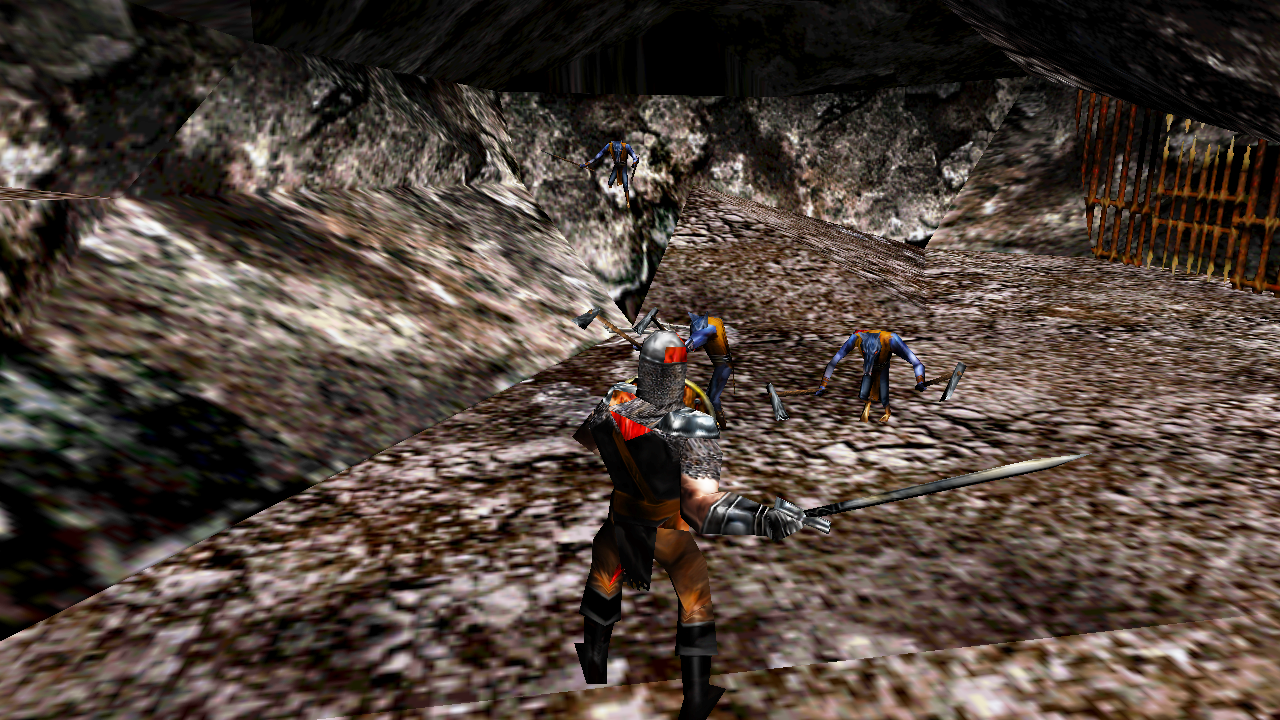
\includegraphics[width=140mm]{../img/DbtS-combat.png}
    \caption{Die by the Sword - ukázka boje}
    \label{obr01:dbts}
\end{figure} 


Jde o jedinou hru, kterou si zde představíme, jež se nevydala cestou omezení množiny stavů meče na konečné množství, ale nabídla hráči skutečně \textbf{jemnou, spojitou kontrolu}. Ta byla umožněna zapojením jednoduchého \textbf{realistického fyzikálního subsystému}, což byl na tehdejší dobu úkaz vskutku nevídaný vzhledem k hardwarovým omezením, v jejichž rámci bylo nutno operovat.

\textbf{Backend hry} umožňoval \textbf{plně volný pohyb} všech objektů třímaných herní postavou (postava mohla např. v jedné ruce držet meč a ve druhé štít či druhý meč), přičemž tělo postavy bylo \textbf{procedurálně animováno} (další na tuto dobu vzácný úkaz), aby poloha jejích rukou s polohou objektů korespondovala.

Tento přístup k implementaci přinesl některé \textbf{zajímavé důsledky}. Hra nepotřebovala implementovat dedikovanou mechaniku pro blokování nepřátelských úderů, stačilo meč napolohovat tak, aby tomu nepřátelskému stál v cestě. Podobným způsobem zde byl nepřeberný prostor pro další zajímavé techniky, vyvíjené a zdokonalované plně hráčskou komunitou. Dále, díky obecnosti systému nebyl problém mít nepřátele všech představitelných tvarů a velikostí - dokud měl nepřítel hmotné tělo, mohli jste ho mečem trefit; dokud měl vhodnou končetinu, mohl sám držet zbraň. Spojením se systémem procedurální animace nestvůrám bylo možné velmi efektně odsekávat kusy těla a kochat se jejich zvýšenou nemotorností\footnote{případně rovnou neschopností hráče zranit, pokud byla odseknuta končetina třímající zbraň}. K dovršení dojmu vás hra nechala chopit se odseknuté končetiny jako zbraně, stále při stejném ovládání, jaké vám nabídl meč.

Kamenem úrazu pro hru však nesporně bylo \textbf{ovládání}. Tvůrci hry si byli zřejmě vědomi, o jak náročnou výzvu vyžadující dlouhodobý výzkum v případě této hry jde, a nabídli hned několik velmi odlišných metod vstupu pro udání pohybu zbraně:
\begin{itemize}
    \item \textbf{Numerická klávesnice}\footnote{V době vzniku hry nebyl grafický operační systém ovládaný myší běžnou součástí výbavy každého hráče. Od her se očekávalo, že budou podporovat možnost ovládání čistě pomocí klávesnice.} - Obdélník číselných kláves symbolizoval obdélník obrazovky, stisknutí dvou kláves (poloh na obrazovce) v rychlém sledu znamenalo švih mečem z jedné polohy na druhou.
    \item \textbf{Myš} - Myší bylo možné udávat pohyb spojitým způsobem. Poloha kurzoru na obrazovce se mapovala na polohu v herním světě, kam se má švihem meč přesunout. 
    \item \textbf{Nahrávky} - Ve hře byl obsažen dedikovaný nástroj umožňující pomocí časové osy a klíčových snímků - způsobem známým z profesionálního softwaru pro tvorbu animací - vytvářet a editovat vlastní zcela libovolné pohyby zbraně. Hotové nahrávce bylo následně možné přiřadit klávesu, jejímž stisknutím ji postava ve hře přehrála. 
\end{itemize}   
Přes značné úsilí, které tvůrci této oblasti věnovali, stalo se ovládání hlavním předmětem hráčské kritiky. Mnoho hráčů si stěžovalo, že je hra jeho vinou nadmíru těžká, případně že si zkrátka \textbf{nehodlají na neotřelý způsob ovládání zvykat}. Přestože hra byla značně oceněna profesionálními kritiky, mezi širokou herní veřejností se jí výrazných ohlasů nedostalo. Kromě datadisku Limb from Limb se již na její odkaz žádná další hra nepokusila navázat, pokud je autorovi této práce známo.

\bigbreak
Celkově vidíme, že hra přinesla systém poskytující \textbf{dodnes nepřekonanou flexibilitu}, nemající problém s nepřáteli všech tvarů, sofistikovanou interakcí s prostředím a umožňující vydatnou dávku emergentního gameplaye. Kamenem úrazu se jí však stalo ovládání. Celkově hra ukázala, že \textbf{návrh ovládání} pro takto flexibilní systém \textbf{je těžký problém}, který vyžaduje více výzkumu.

\subsection{Mount\&Blade}

Kultovní klasikou je Mount\&Blade \cite{MountAndBlade}. První verzi této hry vydalo turecké studio TaleWorlds v roce 2008, později se hra pro velkou oblíbenost mezi hráči dočkala datadisku Warband a velmi nedávno i druhého dílu Bannerlord, který mnoho mechanik hrubě nastíněných v původní hře dále rozvádí a prohlubuje. My se zde budeme věnovat prvnímu dílu, který je v kombinaci s datadiskem Warband i v dnešní době mezi hráči velmi oblíbený a materiálů pro analýzu nám poskytne zcela dostatečné množství.

Jde o \textbf{sandbox} s \acs{RPG} prvky, kde se hráč ujímá role vůdce žoldnéřské skupiny. V jeho kůži putuje od království ke království, verbuje vojáky, plní úkoly pro okolní šlechtice a účastní se po jejich boku bitev se šlechtici znepřátelených zemí. Svět je velmi silně inspirován středověkou Evropou, nenajdeme zde žádnou magii. Nepřáteli jsou výhradně lidé. 

\begin{figure}[ht]\centering
    \center
    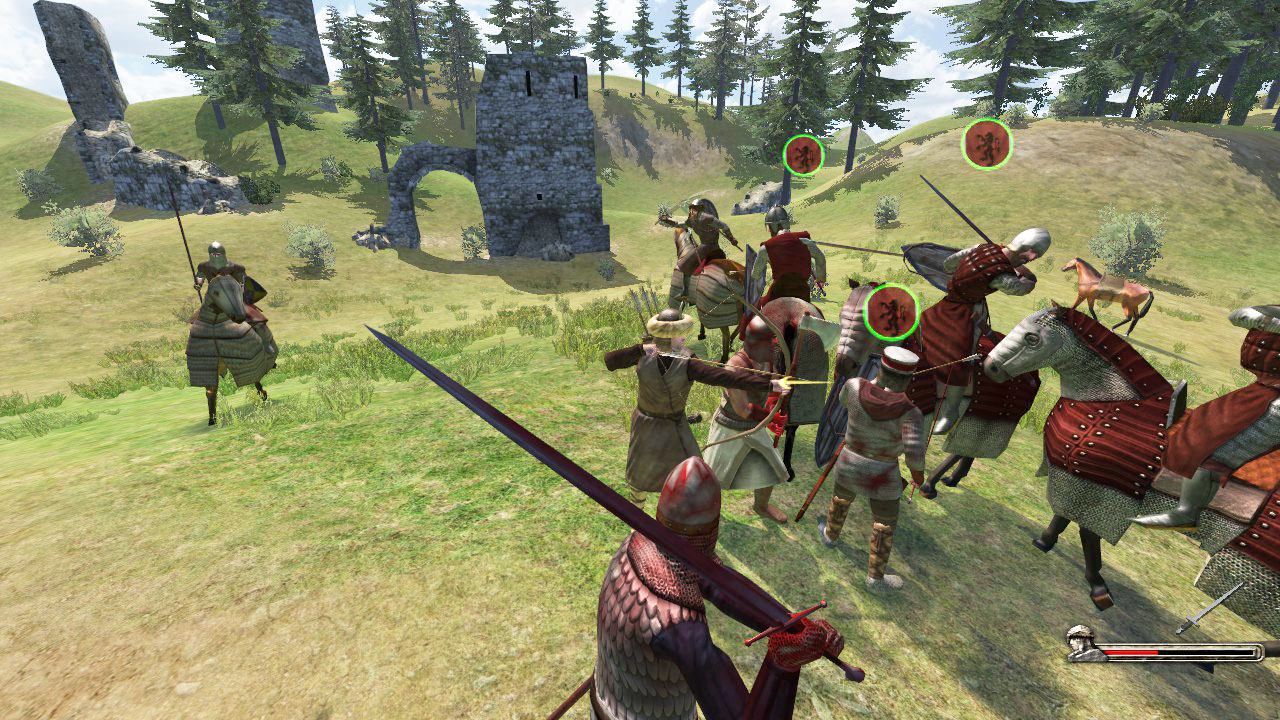
\includegraphics[width=140mm]{../img/MountAndBlade-combat.jpg}
    \caption{Mount\&Blade - ukázka boje}
    \label{obr01:mountandblade}
\end{figure} 

Ovládání vlastní hráčské postavy zde tvoří pouze polovinu skládačky bojového systému - tou druhou je udílení rozkazů zverbovaným vojákům. V bitvách se zde střetávají typicky vyšší desítky až nižší stovky bojovníků spřátelených a nepřátelských. \textbf{Hráčská postava je zde pouze jedním z mnoha} - počítačem řízení bojovníci mají shodné možnosti pohybu i ovládání zbraně a podléhají stejnému systému \acs{RPG} progrese. 

Jak tedy vypadá ovládání zbraně? Každá zbraň má definovanou \textbf{množinu útoků}, které lze provádět. Hráč stiskem tlačítka myši zahájí nápřah, dle polohy kurzoru je vybráno, který z útoků bude vykonán (např. nápřah nad hlavou kurzorem uprostřed nahoře, bodnutí kurzorem uprostřed obrazovky apod.), následně uvolněním tlačítka myši je útok vykonán.

Zbraní najdeme více druhů - meče, sekery, kyje, kopí a další. Útočné zóny jsou napříč zbraněmi shodné, pouze \textbf{některé zóny u některých zbraní chybí} (meč poskytuje všechny, kyj neumožňuje bodání, s kopím lze pouze bodat apod.). Animace, která se přehraje pro útok v dané zóně, je však unikátní pro daný typ zbraně\footnote{Nedochází k žádnému náhodnému výběru, danému páru \textit{zbraň - útočná zóna} přísluší vždy právě jedna pevně daná animace.}.

Druhým typem akce, který lze vykonávat, je \textbf{blokování}. Je-li hráč vybaven štítem, stačí držet stisknuté levé tlačítko myši a postava je kryta proti veškerým úderům, které na ni míří zepředu. Chce-li však postava provést útok se zbraní, musí nejprve kryt přerušit, čímž ochrany pozbyde. Dalším omezujícím faktorem je omezená odolnost štítu - utrží-li štít určité množství \acs{dmg}, je zničen a postava ho zahodí. Čímž přijde na řadu obtížnější situace - blokování pomocí zbraně. Zde se opět dostáváme k využití úderových zón - zkrátka zóna, ve které obránce blokuje, musí odpovídat zóně útočníka - jinak k vyblokování úderu nedojde.

Prvkem, který umocňuje hráčův dojem realističnosti, je způsob \textbf{výpočtu zranění}. Hra se obecně nepokouší o realistickou fyzikální simulaci, avšak způsobené zranění je přesto determinováno kombinací mnoha faktorů, které realistické chování účinně aproximují - zmíníme rychlost zbraně, délku její dráhy apod. . Dále je využíváno jemné detekce kolizí. Zaprvé k tomu, aby se určila zasažená část těla - různým částem těla postavy odpovídá různý kus zbroje, která určuje, jakou mírou má zranění být redukováno. Zadruhé, zranění je velmi silně redukováno, pokud při své cestě zbraň prošla skrze zeď či jiný prvek okolního prostředí. 

Nyní rámcově víme, jak bojový systém funguje. Pojďme se tedy podívat na \textbf{benefity}, které z této implementace plynou. Vidíme, že hře se \textbf{podařilo najít kompromis} slučující některé prvky, které by se z naší předchozí anylýzy mohly zdát vzájemně protichůdné.
\begin{itemize}
    \item \textbf{Jednoduchost X Pocit kontroly} - Hráčova kontrola nad mečem je sice omezená na výběr z malé množiny úderových zón, těch je však stále dostatečné množství, aby pokryly většinu způsobů útoku, které by běžnému hráči rozumně mohly přijít na mysl. Protože správný výběr útoku má velmi reálný efekt na jeho úspěch, hráč je motivován svou možnost volby vzít plně na vědomí a ne ji přejít jako pouhý kosmetický detail. 
    \item \textbf{Uniformní ovládání X Osobitost jednotlivých zbraní} - Ovládání odpovídá napříč zbraněmi totožné šabloně, konkrétní provedení vyžádaného útoku se však mezi typy zbraní liší dostatečně, aby to mělo citelný efekt na pocit ze hry. Rovněž fakt, že pro každý pár \textit{zbraň - typ útoku} existuje pouze jediná pevně daná animace, umocňuje předvídatelnost, která hráči umožňuje zbraň rychle pochopit a být si intuitivně vědom jejích specifik.
\end{itemize}

Systém však přinesl i některá \textbf{nepohodlí a promarněné příležitosti}:
\begin{itemize}
    \item \textbf{Ovládání kamery} - Pohyb myši plní současně dvě nesouvisející role - ovládání natočení kamery a výběr zóny útoku - což se ne vždy dobře slučuje. Nastávají situace, kdy hráč, aby vybral směr útoku, musí pohled přetočit pryč z místa zasluhujícího pozornost, což může vést k mírnému zmatení.  
    \item \textbf{Emergentní gameplay} - Bojový systém je uzavřená bublina, která s okolními mechanikami ani sama se sebou neinteraguje natolik, aby vznikl prostor pro vznik zajímavých interakcí, jaké tvůrci hry úmyslně neplánovali.
    \item \textbf{Flexibilita} - Do hry by bylo obtížné přidat např. specifický typ nehumanoidních postav - celý systém útočných zón by se musel překopat, aby byl boj s nimi schopen poskytnou stejně realistický zážitek jako boj s lidmi.
\end{itemize}

Celkově tedy vidíme, že hře se podařilo najít \textbf{zajímavý kompromis mezi realističností, pocitem kontroly, a hráčskou přívětivostí}. O jeho kvalitách svědčí dlouhodobě velmi pozitivní ohlasy hráčské komunity. Bylo toho však dosaženo obětováním jisté vnitřní flexibility - systém velmi dobře vystihuje boj lidí s lidmi, použití zbraně k jakémukoliv jinému účelu by však žádalo jeho významné překopání. 


\subsection{Kingdom Come: Deliverance}
Poslední hrou, kterou zmíníme, je Kingdom Come: Deliverance \cite{KCD}, vydáné roku 2018 českými Warhorse Studios. Jde o akční \acs{RPG} odehrávající se v českém Posázaví roku 1403. Jedním z hlavních důrazů hry byla \textbf{historická věrnost a celková realističnost zážitku} - z tohoto rozhodnutí plynou přirozeně dalekosáhlé důsledky pro bojový systém.

\begin{figure}[ht]\centering
    \center
    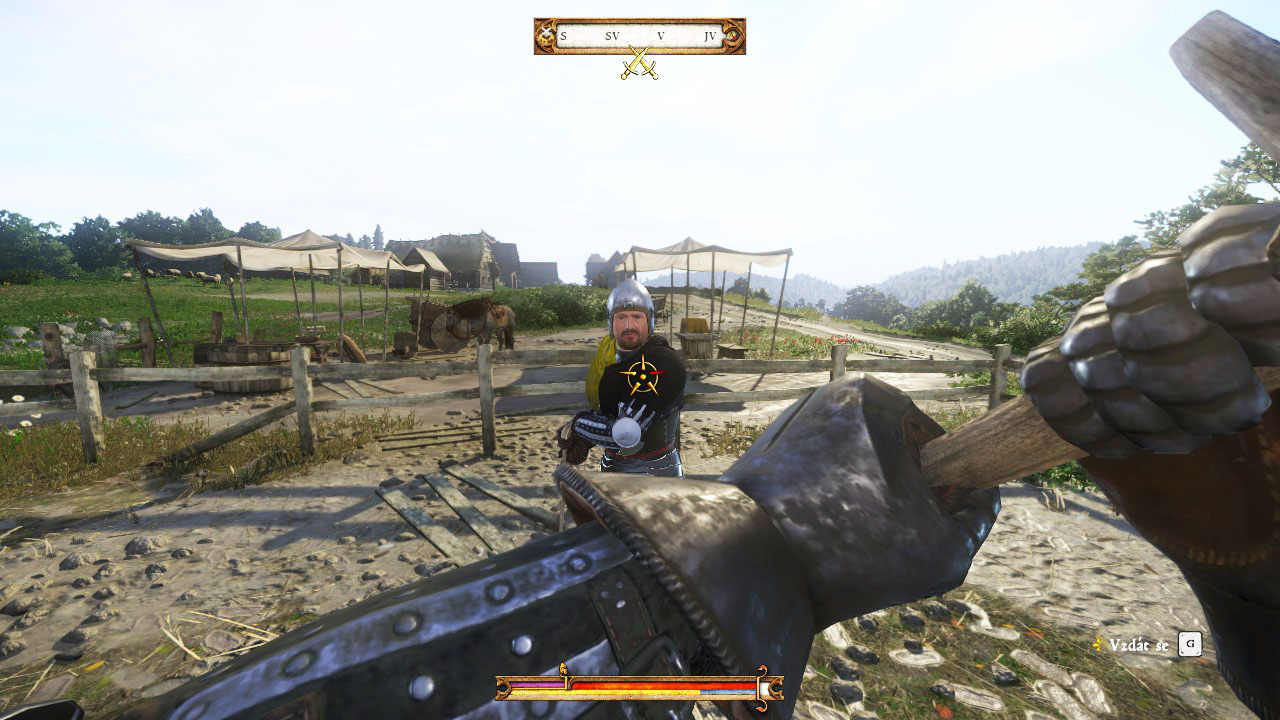
\includegraphics[width=140mm]{../img/KCD-combat.jpg} 
    \caption{Kingdom Come: Deliverance - ukázka boje}
    \label{obr01:kcd}
\end{figure} 

Některé prvky hra sdílí s předchozí představenou Mount\&Blade. Hráč je zde rovněž pouze \textbf{jedním z mnoha}, lidští \acs{NPC}s mají totožné možnosti pohybu, ovládání meče a vztahuje se na ně i stejný systém RPG progrese.

Tím podobnosti nekončí. Přistoupíme-li k boji samotnému, rovněž zde najdeme velmi podobnou množinu \textbf{útokových zón}, mezi kterými hráč vybírá pohybem myši. Co se však již liší, je způsob, jakým je útok vykonán. Nenajdeme zde samostatnou akci pro zahájení nápřahu. Místo toho je boj rozlišován jako specifický stav, ve kterém se hra může nacházet - dokud boj trvá, postava je napřažena neustále, ve směru dle aktuálně vybrané útokové zóny. Stisknutím tlačítka myši je útok rovnou vykonán. 

Výrazným rozdílem proti Mount\&Blade je pohled z 1. osoby, doprovázený mechanikou \textbf{uzamčení na protivníka}. Ta zajišťuje, že je na protivníka neustále zaměřena kamera, výpady jsou prováděny směrem proti jeho pozici apod. . Tím je hráč zbaven námahy provádění mechanických úkonů, které by v reálném světě pro jeho postavu byly samozřejmé, což přispívá k celkově plynulejšímu a intuitivnějšímu dojmu z ovládání. 

Mechanikou, která na uzamykání na protivníka závisí, je \textbf{blokování}. To je zde zpracováno jako časovací prvek. V okamžiku, kdy protivník útočí, se hráči na chvíli uprostřed útokové růžice zobrazí zelený symbol štítu - stisknutím tlačítka blokování tehdy a právě tehdy je úder vyblokován. Držením zbraně v zóně, do které probíhá útok, je blokovací okno zvětšeno. Pokud je postava vybavena štítem, rovněž to má na velikost blokovacího okna pozitivní vliv. Příležitostně může být jedodušší místo riskantního pokusu o blokování zkrátka popojít dozadu či na stranu a úderu se vyhnout. 

Prvkem, o který Mount\&Blade letmo zavadilo, je \textbf{zbroj bojovníků}. Kingdom Come zde jde mnohem dál a představuje pokročilý systém umožňující oblékání po vrstvách. Přesně jako v realitě na sobě bohatý šermíř může mít obyčejnou civilní tuniku, přes ní prošívanici tlumící svými mnoha vrstvami tuhé látky tupé údery, přes ty kroužkovou zbroj, a dovršit plechovými pláty. Chudý branec si mezitím vystačí s prošívanicí. Výpočet zranění pak odpovídá vlastnostem oblečení kryjícího zasaženou část postavy. Toto vše je doplněno i vizuální stránkou - veškeré vrstvy oblečení jsou přes sebe na modelu postavy korektně skládány. Co dokáže okořenit herní zážitek, je omezení zorného pole na průduchy, které hráčově postavě poskytuje uzavřená přilba. 

Naprosto zásadní mechanikou je \textbf{správa výdrže}. Každá akce (útok, blokování apod.) spotřebovává její díl, stejně tak i utržené zranění. To až do takové míry, že bojovníkovi oděnému do těžké zbroje nepřátelské zásahy mnohdy ubírají téměř pouze výdrž. Jakmile bojovník žádnou výdrž nemá, je zranitelný - ne jen, že nemůže provádět akce na svou obranu - vše, co již zásah nemůže ubrat z výdrže, ubere z jeho \acs{HP}. Ubranými životy se hráči snižuje i maximální množství výdrže, které může zregenerovat a dostává se tím do dlouhodobé nevýhody. Boj se tak stává složitou hrou taktizování a zvažování priorit.\footnote{Neohrabané nakládání s výdrží může vypadat například tak, že bojovník zažene protivníka sérií úderů do úzkých, jen aby zjistil, že se tím příliš vyčerpal a není schopen ho dorazit. O okamžik později protivník využije jeho zranitelnosti a situace se obrací.}  

Celý bojový systém je rovněž úzce svázán s \textbf{\acs{RPG} progresí}. Základem je zběhlost v použití jednotlivých typů zbraní a v blokování. Ta se projevuje mnoha způsoby - od celkové šermířské finesy pozorovatelné na animaci útoku, po velikost časového okna pro blokování \footnote{Zvyšuje se s bojovníkovou schopností blokovat, snižuje s nepřítelovou schopností útočit.}. Dále je například možné odemykat specielní techniky - ty mohou následně být použity provedením specifické sekvence úderů (do specifických útočných zón) a oproti běžným úderům poskytují nějaký stanovený bonus.

Za možnou slabinu bojového systému lze považovat \textbf{boj proti více protivníkům}. Zatímco v boji 1v1 je uzamykání na protivníka vítaným pomocníkem, je-li protivníků více, nutnost soustředit se na jednoho z nich značně přispívá k celkovému zmatku a nepohodlí. Dalo by se namítat, že zmatek a nepohodlí neodlučitelně patří k situaci, jakou je boj proti přesile. Rovněž, jak jsme si nastínili v \ref{organizedFightingIrlSubsection}, v reálném světě často jedinou rozumnou možností, jak přesilu přemoci, skutečně je rozdělit ji a svést boj s jednotlivci - k čemuž přesně tento systém vybízí. Z celkových hráčských ohlasů je však zřejmé, že toto nepatří mezi ty aspekty realizmu, o které má herní publikum zájem.

\pagebreak

Nyní by čtenář měl být rámcově seznámen s bojovým systémem. Pojďme si tedy shrnout, které věci se \textbf{obzvláště zdařily}:

\begin{itemize}
    \item \textbf{Značná hloubka systému} - Systém výdrže, spolu s pohybem postav a výběrem útokových zón vytvářejí značný prostor k taktickému jednání. Jednání protivníka je dostatečně sofistikované, aby pro hráče nebylo nikdy dokonale průhledné, avšak fakt, že je vázán stejnými systémy jako hráč, dává značný prostor k pokusům o jeho předvídání. Systém progrese nabízí další zajímavé možnosti, jak průběh boje ovlivnit. 
    \item \textbf{Plynulý dojem z boje} - Systém hráči velmi dobře komunikuje herní stav - hráč přesně ví, co se děje a jak si v boji vede. Zároveň systém na uživatelské vstupy reaguje dostatečně responzivně. Díky tomu je hráč schopen utvářet a realizovat rozhodnutí srovnatelně rychle, jako kdyby bojoval v reálném světě.
    \item \textbf{Ovládání kamery} - Kamera je uzamčena na protivníka. Pro vybrání útokové zóny není třeba žádný nežádaný pohyb kamery. I kdyby však k uzamčení kamery nedocházelo, problém by zde nevyvstával ani zdaleka tak výrazně jako v Mount\&Blade. Důvodem je fakt, že útoková zóna pro bodání (uprostřed) je zde specielním případem, který se vybírá stisknutím pravého tlačítka myši. Každá ze zbylých zón odpovídá jednomu ze směrů růžice, pohyb kurzoru nutný k jejich rozlišený je tedy velmi drobný. 
    \item \textbf{Reflexe narativní progrese} - Minimálně stejnou mírou jako na hráčské dovednosti závisí bojová schopnost postavy i na její \acs{RPG} progresi. Jelikož progrese hráče skrze \acs{RPG} systémy je spjatá s jeho progresí v narativu hry, je zde citelně zredukován prostor pro vznik disonance jakou jsme popsali v \ref{moreControlBenefitsSection}.
\end{itemize}

Najdeme zde i některé \textbf{nevýhody}:
\begin{itemize}
    \item \textbf{Interakce s prostředím} - Bojový systém je koncipovaný čistě pro souboj s protivníkem. Mimo souboj lze provádět pouze jediný stále stejný útok. Navíc objekty prostředí na rány meče ani nejsou schopny jakkoliv reagovat.  
    \item \textbf{Boj s více protivníky} - Nutnost uzamčení kamery na jednoho protivníka vede ke zmatku.
    \item \textbf{Flexibilita} - Přidat do hry např. specifický typ nehumanoidních postav je nanejvýš obtížné. Pro optimální zážitek by bylo nutné pro boj s novým protivníkem vytvořit i zcela nový systém útokových zón s novými animacemi, specielními technikami apod.\footnote{Počet takových systémů by rostl kvadraticky s počtem typů postav, počítáme-li, že tyto postavy mohou bojovat i vzájemně mezi sebou.}. O obtížnosti takového snažení ostatně mnoho vypovídají hráčské ohlasy k datadisku, kterým do hry jako nepřátelé byli přidáni psi.  
\end{itemize}

Celkově vidíme, že se hře podařilo vytvořit systém vyznačující se značnou hloubkou, který hráči umožňuje vynášet rozhodnutí podobně komplexní\footnote{Myšleno, že z pohledu typického hráče se tváří dojmem podobné komplexity. Ne že skutečně jsou.} jako při reálném boji a podobně rychle, jako je nutné při reálném boji - to vše při grafickém výstupu, který se ve všech ohledech velmi blíží zachycení reálného středověkého boje. Není tedy divu, že je hra obecně považována za velmi dobré zachycení realistického středověkého boje. Cenou za to však je celkově nízká flexibilita a nemožnost meč použít k jakémukoliv jinému účelu, než je boj proti lidským protivníkům.

\subsection{Shrnutí}

Existuje mnoho dobrých důvodů, proč by hráč měl mít zájem o přímější kontrolu nad chladnou zbraní, poskytnout mu ji však je obtížný a nevděčný úkol, jehož splnění se neobejde bez kompromisů.  

Největším problémem se zdá být \textbf{ovládání}. Všechny hry, které jsme si představili, jež měly mezi hráčskou komunitou úspěch, se ubíraly cestou \textbf{omezení množiny stavů}, ve kterých se zbraň může nalézat, na nemalou ale \textbf{konečnou} velikost. Tato cesta se zdá v reálném světě fungovat, neposkytuje však vysokou flexibilitu, bojový systém musí být hardcodován pro lidské nepřátele a nenabízí vysoké možnosti emergentního gameplaye. 

O plně flexibilní systém umožňující \textbf{volný pohyb zbraně} a boj jakýchkoliv dvou entit majících končetiny schopné zbraň třímat se pokusilo Die by the Sword \cite{DieByTheSword} - to se však stalo živoucím důkazem, že navrhnout použitelné ovládání pro takový typ systému je \textbf{těžkým problémem}, jehož uspokojivé řešení si vyžaduje více výzkumu. Pokud je autorovi této práce známo, žádné výzkumné snahy v tomto směru dosud nebyly vyvinuty.

%------------------------------------------------------------------------------------------------------------------------------------------------------------------------------------------------------------------------------------------------------------%
 % xxxxxxxxxxxxxxxxxxxxxxxxxxxxxxxxxxxxxxxxxxxxxxxxxxxxxxxxxxxxxxxxxxxxxxxxxxxxxxxxxxxxxxxxxxxxxxxxxxxxxxxxxxxxxxxxxxxxxxxxxxxxxxxxxxxxxxxxxxxxxxxxxxxxxxxxxxxxxxxxxxxxxxxxxxxxxxxxxxxxxxxxxxxxxxxxxxxxxxxxxxxxxxxxxxxxxxxxxxxxxxxxxxxxxxxxxxxxxxxxxxxxxxxx %
%------------------------------------------------------------------------------------------------------------------------------------------------------------------------------------------------------------------------------------------------------------%


\section{Alternativní ovladače} \label{alternativeControllers}

Jak jsme si nastínili v předchozí sekci, \textbf{ovládání} je těžkým problémem, který musí vyřešit každá hra, která se hráči pokouší poskytnout nad zbraní větší kontrolu. V dosavadní části práce jsme však brali v úvahu výhradně běžné ovladací periferie - počítačovou myš a klávesnici, popř. ovladač u herní konzole. Jejich společným znakem je dvourozměrný charakter informace, jíž poskytují. Hlavní problém pak plyne z potřeby namapovat tuto 2D hodnotu na 3D polohu meče. 

Existuje však mnoho dalších, méně obvyklých způsobů ovládání. V této sekci se podíváme na několik z nich, které mají potenciál posloužit jako zdroj 3D vstupu.

\subsection{Virtuální realita} \label{VRControllers}

Očividným místem, kde můžeme najít ovladač poskytující 3D vstup, je virtuální realita (dále jen \acs{VR}). Tato oblast během posledního desetiletí prochází bouřlivým vývojem. Najdeme zde mnoho konkurujících si herních systémů, každý se svými silnými a slabými stránkami. Jádro libovolného z nich však tvoří headset a dvojice ovladačů, vždy plně trackující svůj pohyb v prostoru.  

Jde tedy o místo, které k použití jemně ovladatelné, fyzikálně simulované chladné zbraně přímo vybízí. A her, jež ji hráči poskytnou, tu skutečně najdeme nemálo - zmíníme např. Blade and Sorcery \cite{BladeAndSorcery} či GORN \cite{Gorn}.

Ať už se však \acs{VR} zdá jakkoliv ideálním místem pro chladnou zbraň, přináší své vlastní limitace a nevýhody. Známým problémem, který trápí většinu \acs{VR} her, je hráčova limitovaná \textbf{schopnost pohybu po herním světě}. Jemná kontrola nad zbraní je tedy vykoupena obětí jiného z aspektů realistického boje. 

Dalším problémem je \textbf{disonance mezi polohou ovladače v reálném a polohou meče v herním světě}. Obecně se hry snaží držet tyto dvě synchronizované, problém však nastane, jakmile meč zaznamená \textbf{kolizi}. V takové situaci zpravidla ovladač spustí nepříjemné vibrace, nic více však není v jeho silách. Dle hráčských výpovědí takovými situacemi velmi trpí imerze a celkový herní zážitek. 

Pro situaci kolize se statickými objekty herní scény zřejmě neexistuje dobré řešení. V praxi hojně užívaným řešením pro kolize s nepřátelskými zbraněmi je zkrátka prioritizovat pohyb hráčovy zbraně a nepřátele učinit druhořadými entitami, jejichž zbraň musí té hráčově vždy ustopit. Takový přístup má přirozeně dalekosáhlé následky na gameplay a není použitelný v multiplayeru. 

Vidíme tedy, že boj s chladnými zbraněmi ve \acs{VR} je osobitým polem, které nabízí velmi odlišné silné stránky, výzvy a oblasti hodné prozkoumání, než jeho podoba pro klasické PC.

V této práci se však touto problematikou nebudeme hlouběji zabývat, protože stále jde o způsob hraní poměrně \textbf{málo rozšířený} mezi hráčskou populací. Konkurenční boj tlačí ceny dolů, stále je zde však velmi mnoho hráčů, pro které je \acs{VR} cenově nedostupná. Limitující mohou být i technické faktory - např. rozlišení displejů používaných v současných headsetech či jejich nízká obnovovací frekvence mohou pro některé hráče z \acs{VR} učinit velmi nepříjemný zážitek. 

\subsection{Wii Remote} \label{wiiRemoteSubsection}

Mnoho problémů, kterými \acs{VR} trpí, plynou z jeho základní premisy plně přenést hráče do virtuálního světa. Co kdybychom se tedy zbavili headsetu a nechali si pouze ovladač jako doplněk k periferiím klasického PC?

V takovém případě by náš výsledek mohl vypadat zhruba podobně jako konzole Nintendo Wii. Pro tu byla vydána řada her založených na použití jejího ovladače Wii Remote - pro nás je důležitá zejména \textbf{The Legend of Zelda: Skyward Sword} \cite{ZeldaSkywardSword}. Jednou z ústředních mechanik této hry je jemně ovladatelný meč - používaný jak k boji, tak k řešení logických hádanek. Z dobových recenzí (\cite{SkywardReviewNintendolife} \cite{SkywardReviewIgn}) je zřejmé, že vše funguje velmi dobře. 

Wii je v dnešní době zastaralou platformou, pro kterou nemá smysl vyvíjet nové hry, avšak samostatný ovladač Wii Remote lze ve výprodeji pořídit vcelku levně\footnote{Narozdíl od ovladačů pro moderní \acs{VR} headsety, které typicky samostatně prodejné nejsou.} a díky komunitnímu úsilí \cite{WiiRemoteUnityAPI} by neměl být problém s jeho použitím jako ovladač pro PC hru v enginu Unity. Stále však nelze očekávat, že většinový hráč bude ochotný kvůli naší hře ovladač pořizovat, a i mimo to, vydání komerční hry pro PC platformu hlásící se k jeho podpoře by mohlo být velmi obtížné po právní stránce.

Jistě má však tento ovladač potenciál posloužit v průběhu tvorby hry jako \textbf{interní nástroj} pro testování konceptů, či jako kontrolní bod, vůči kterému lze srovnávat experimentální alternativy.

\subsection{Pohybové senzory ve smartphonu}

Alternativou, která má potenciál vyřešit problém dostupnosti, je použití chytrého telefonu jako ovladače. Smartphony jsou typicky vybaveny širokou škálou senzorů, s jejichž pomocí by monitorování pohybu ve 3D prostoru nemělo hypoteticky činit problém. Stačilo by tedy vytvořit aplikaci, která se po síti spáruje s herním PC a následně mu bude posílat výstupy těchto senzorů?

V praxi však kvalita výstupů těchto senzorů není na přijatelné úrovni \cite{SmartphoneSensorsEvaluation} - typicky trpí na silné zašumění, rovněž je problémem extrémní fragmentace mobilního trhu, kdy každý jednotlivý model telefonu produkuje šum jiným způsobem a vyžaduje jinou ruční kalibraci. Tyto limitace by mohly být překonatelné - ve spřízněných oblastech se např. ukazují jako velmi nápomocné metody strojového učení \cite{AccelerometerStepDetectionUsingML} - avšak k tomu je třeba mnoho dalšího výzkumu, a ten postupuje pomalu.

\subsection{Shrnutí}
Provedli jsme zamyšlení nad alternativními způsoby ovládání, které by usnadnily náš úkol poskytnout hráči intuitivní a jemnou kontrolu nad mečem. Ovladače pro \acs{VR} jsou očividným řešením, dokonce již existuje několik her, které jejich velmi dobrou použitelnost demonstrují v praxi. Stále však jde o malý trh, který se jen velmi pomalu rozšiřuje do mainstreamu - omezíme-li se na něj, citelně se zůží potenciální hráčské publikum.

Podobným případem je ovladač pro konzoli Nintendo Wii. Jde o praxí osvědčené a relativně levně dostupné zařízení, jeho podpora u komerční PC hry by však znamenala právní risk.

Problém dostupnosti by se dal vyřešit emulací takového ovladače pomocí běžného chytrého telefonu. Moderní mobilní zařízení jsou vybaveny škálou senzorů, s jejichž použitím by to neměl být problém. V praxi však jsou senzory náchylné na šum, narážíme rovněž na fragmentaci mobilního trhu, každý model trpí na šum trochu jiným způsobem. Dovedení této metody do použitelného stavu by vyžadovalo další výzkum, kterého se příliš nedostává.

Docházíme tedy k závěru, že bude nejlépe, když naší hře umožníme podporovat klasické ovládání pomocí klávesnice a myši. Možnost podporovat někdy v budoucnu i \acs{VR} ovladač neuškodí, nejde však o prioritu.

\section{Shrnutí}

Uvedli jsme čtenáře do problematiky boje s chladnou zbraní v reálném světě, tento náhled jsme následně zkontrastovali s tím, jak je tato problematika zachycena ve videohrách.

V reálném světě jde o extrémně komplexní oblast, která za sebou má mnoho tisíciletí vývoje, nespočet technik vedoucích k jedinému cíli - vyřadit protivníka z bojeschopného stavu dříve než on vás. Naprostými základy jsou orientace na bojišti, správná technika pohybu, obratné a kreativní použití zbraně, a předvídání protivníka. V případě hromadného boje pak rovněž koordinace a disciplína vojenského celku. 

Ve videohře chladná zbraň typicky figuruje jako ''černá skříňka'' - hráči je poskytnuto jediné tlačítko - \textbf{Zaútoč!} - jeho stisknutím postava provede útok jak sama uzná za vhodné. Výhodami tohoto systému jsou jednoduchost použití a univerzální aplikovatelnost i pro škálu velmi vzájemně odlišných zbraní. Má-li boj s chladnou zbraní sloužit jako nosná herní mechanika, hloubka mu je typicky dodávána důrazem na pohyb, přehled o bojové situaci a přesné časování, dále kombinací s dalšími systémy (magie, lektvary, pasti), v neposlední řadě kreativním designem nepřátel.

Takový systém tedy pěkně vystihuje některé z aspektů, které hrají roli v reálném světě. Ten, který je pro typického laika nejzjevnější - totiž ovládání zbraně - je však ponechán zcela mimo hráčovu přímou kontrolu. Hra, které by se zdařilo poskytnout hráči nad zbraní bezprostřední kontrolu, by tím mohla získat mnoho benefitů - mimo zjevné atraktivity plynoucí z neohranosti konceptu například taková zbraň má potenciál stát se vděčným zdrojem emergentního gameplaye.

Představili jsme si podrobněji několik her, které se o dosažení tohoto cíle pokoušely. Oba komerčně úspěšní zástupci (\cite{MountAndBlade} \cite{KCD}) se ubírali cestou omezení množiny stavů, ve kterých se meč může nalézat, na nemalou ale konečnou velikost. Jejich společným znakem bylo velmi dobré ztvárnění boje člověka proti člověku, avšak vykoupené nízkou flexibilitou znemožňující zakomponování nehumanoidních nepřátel či použití meče k čemukoliv jinému než přímočarému boji.

Protipólem pak bylo Die by the Sword \cite{DieByTheSword}. To kombinací realistické fyzikální simulace a procedurální animace vytvořilo systém, který nad pohybem meče umožnil spojitou kontrolu a nečinil mu problém zápas libovolných entit vybavených libovolným počtem končetin třímajících meč. Kamenem úrazu se mu však stalo ovládání. Problém plynul z faktu, že tradičně používané ovládací periferie poskytují dvourozměrný vstup, který nelze přímočaře namapovat na 3D polohu a rotaci meče. Pro hry usilující o takovou míru volnosti jako Die by the Sword jde do dnešní doby o těžký problém, pro který nebylo nalezeno uspokojivé řešení - jedinou možností se zdá být výměna myši za drahý \acs{VR} ovladač.
